\documentclass[12pt,a4paper]{ctexart}

\usepackage[a4paper,margin=2.5cm]{geometry}
\usepackage{setspace}
\usepackage{array}
\usepackage{longtable}
\usepackage{graphicx}
\usepackage{fancyhdr}
\usepackage{titling}
\usepackage{enumitem}
\usepackage{amsmath,amssymb}
\usepackage{booktabs}
\usepackage{caption}
\usepackage{float}
\usepackage{hyperref}
\usepackage{listings}
\usepackage[dvipsnames, svgnames, x11names]{xcolor}

\lstset{
	backgroundcolor=\color[rgb]{0.96,0.96,0.96},
	keywordstyle=\color{blue}\bfseries,
	identifierstyle=\color{black},
	commentstyle=\color[rgb]{0,0.6,0},
	stringstyle=\color[rgb]{0.58,0,0.82},
	basicstyle=\small\ttfamily,
	columns=fullflexible,
	breaklines=true,
	captionpos=t,
	tabsize=4,
	morekeywords={},
	emph={self},
	emphstyle=\bfseries\color{Rhodamine},
	frame=lines,
	framesep=1em,
	rulesepcolor=\color{red!20!green!20!blue!20},
	language=Python,
	numbers=left,
	showstringspaces=false,
	numberstyle=\footnotesize,
	extendedchars=false,
	xleftmargin=3em
}

\setlength{\parindent}{2em}
\setlength{\parskip}{0.5em}
\renewcommand{\arraystretch}{1.5}
\linespread{1.3}

\pagestyle{fancy}
\fancyhf{}
\cfoot{\thepage}
\renewcommand{\headrulewidth}{0pt}

% ===== 可修改信息 =====
\newcommand{\schoolname}{数学与统计学院}
\newcommand{\classname}{数学强基2301}
\newcommand{\studentid}{2233210080}
\newcommand{\studentname}{袁浩然}
\newcommand{\teachername}{孟德宇老师}
\newcommand{\labplace}{数学实验中心}
\newcommand{\experimenttitle}{EM 算法解决混合高斯模型聚类问题}
\newcommand{\schoolyear}{2023--2024学年\quad 第二学期}

\begin{document}

\begin{titlepage}
	\centering
	{
\includegraphics[scale=1]{figure1.jpg}}

	\vspace{1.8cm}

	{\heiti\zihao{-1} 机器学习\par}

	\vspace{2.2cm}

	{\zihao{3} 实验报告\par}

	\vspace{1.8cm}

	{\zihao{4} \schoolyear\par}

	\vspace{1.8cm}

	\renewcommand{\arraystretch}{2.0}
	\begin{tabular}{>{\raggedleft\arraybackslash}p{7cm} p{9cm}}
		学\hspace{2em}院： & \schoolname \\
		班\hspace{2em}级： & \classname \\
		学\hspace{2em}号： & \studentid \\
		姓\hspace{2em}名： & \studentname \\
		指导教师： & \teachername \\
		实验地点： & \labplace \\
	\end{tabular}

	\vfill
\end{titlepage}

\section*{实验五：EM 算法解决混合高斯模型聚类问题}

\section*{一、问题描述}
本实验考虑一个带隐变量的无监督聚类任务。给定一组二维观测数据，样本来自 $K$ 个高斯分布的混合，但每个样本属于哪个高斯成分是未知的。目标是使用 EM 算法估计高斯混合模型（GMM）参数，并完成聚类。

根据题目要求，实验重点是手写 EM 过程，不直接调用现成的 GMM 聚类函数。最终输出聚类准确率（通过标签重排后与真实标签比较）以及对数似然曲线。

\section*{二、算法原理}
高斯混合模型可写为：
\[
p(x)=\sum_{k=1}^{K}\pi_k\,\mathcal{N}(x\mid\mu_k,\Sigma_k),\quad \sum_{k=1}^{K}\pi_k=1
\]
其中 $\pi_k$ 是混合系数，$\mu_k$ 和 $\Sigma_k$ 分别是第 $k$ 个高斯成分的均值与协方差。

EM 算法迭代执行两步：
\begin{enumerate}
	\item \textbf{E 步：} 计算后验责任度
	\[
	\gamma_{ik}=\frac{\pi_k\mathcal{N}(x_i\mid\mu_k,\Sigma_k)}{\sum_{j=1}^{K}\pi_j\mathcal{N}(x_i\mid\mu_j,\Sigma_j)}
	\]
	\item \textbf{M 步：} 利用责任度更新参数
	\[
	N_k=\sum_{i=1}^{n}\gamma_{ik},\quad
	\pi_k=\frac{N_k}{n},\quad
	\mu_k=\frac{1}{N_k}\sum_{i=1}^{n}\gamma_{ik}x_i,
	\]
	\[
	\Sigma_k=\frac{1}{N_k}\sum_{i=1}^{n}\gamma_{ik}(x_i-\mu_k)(x_i-\mu_k)^T
	\]
\end{enumerate}

每轮迭代计算一次总对数似然
\[
\mathcal{L}=\sum_{i=1}^{n}\log\left(\sum_{k=1}^{K}\pi_k\mathcal{N}(x_i\mid\mu_k,\Sigma_k)\right)
\]
并用其增量判断收敛。

\section*{三、实验步骤与实现细节}
\begin{enumerate}
	\item 生成二维三簇混合高斯模拟数据，并保留真实标签用于后续准确率评估；
	\item 初始化参数：$\pi_k$ 均匀、均值随机抽样、协方差初始化为样本协方差；
	\item 执行 E 步，计算每个样本属于每个簇的责任度；
	\item 执行 M 步，更新混合系数、均值和协方差矩阵；
	\item 记录每次迭代的对数似然值，直到增量小于阈值或达到最大迭代次数；
	\item 由责任度最大值给出聚类标签；
	\item 由于聚类标签有置换不确定性，采用全排列匹配求最优准确率；
	\item 绘制原始数据图、聚类结果图和对数似然曲线图。
\end{enumerate}

\section*{四、核心代码}
下面列出实现中最关键的 EM 主体结构。

\begin{lstlisting}
class GMMEM:
	def __init__(self, n_components=3, max_iter=1000, tol=1e-6, random_state=7):
		self.n_components = n_components
		self.max_iter = max_iter
		self.tol = tol
		self.random_state = random_state
		self.pi_ = None
		self.means_ = None
		self.covs_ = None
		self.log_likelihood_history_ = []

	def _e_step(self, x):
		n_samples = x.shape[0]
		resp = np.zeros((n_samples, self.n_components))
		for k in range(self.n_components):
			resp[:, k] = self.pi_[k] * multivariate_gaussian_pdf(x, self.means_[k], self.covs_[k])
		row_sum = np.sum(resp, axis=1, keepdims=True)
		row_sum[row_sum == 0] = 1e-12
		resp = resp / row_sum
		return resp

	def _m_step(self, x, resp):
		n_samples, n_features = x.shape
		nk = np.sum(resp, axis=0)
		nk[nk == 0] = 1e-12

		self.pi_ = nk / n_samples
		self.means_ = (resp.T @ x) / nk[:, np.newaxis]

		new_covs = np.zeros((self.n_components, n_features, n_features))
		for k in range(self.n_components):
			diff = x - self.means_[k]
			weighted_diff = resp[:, k][:, np.newaxis] * diff
			cov_k = (weighted_diff.T @ diff) / nk[k]
			cov_k += 1e-6 * np.eye(n_features)
			new_covs[k] = cov_k
		self.covs_ = new_covs

	def fit(self, x):
		self._initialize(x)
		prev_ll = None
		for _ in range(self.max_iter):
			resp = self._e_step(x)
			self._m_step(x, resp)
			ll = self._log_likelihood(x)
			self.log_likelihood_history_.append(ll)
			if prev_ll is not None and abs(ll - prev_ll) < self.tol:
				break
			prev_ll = ll
		return self
\end{lstlisting}

\section*{五、实验结果与分析}
实验结果显示，对数似然曲线随迭代单调上升并最终趋于平稳，说明 EM 过程正常收敛。聚类结果图中，三个簇在平面上被较好地区分，估计均值基本落在各簇中心区域。

按题目要求，本实验输出了聚类准确率（采用最优标签映射后计算）。从结果看，准确率较高，说明手写 EM-GMM 能够较好恢复数据潜在分布结构。

\begin{figure}[H]
	\centering
	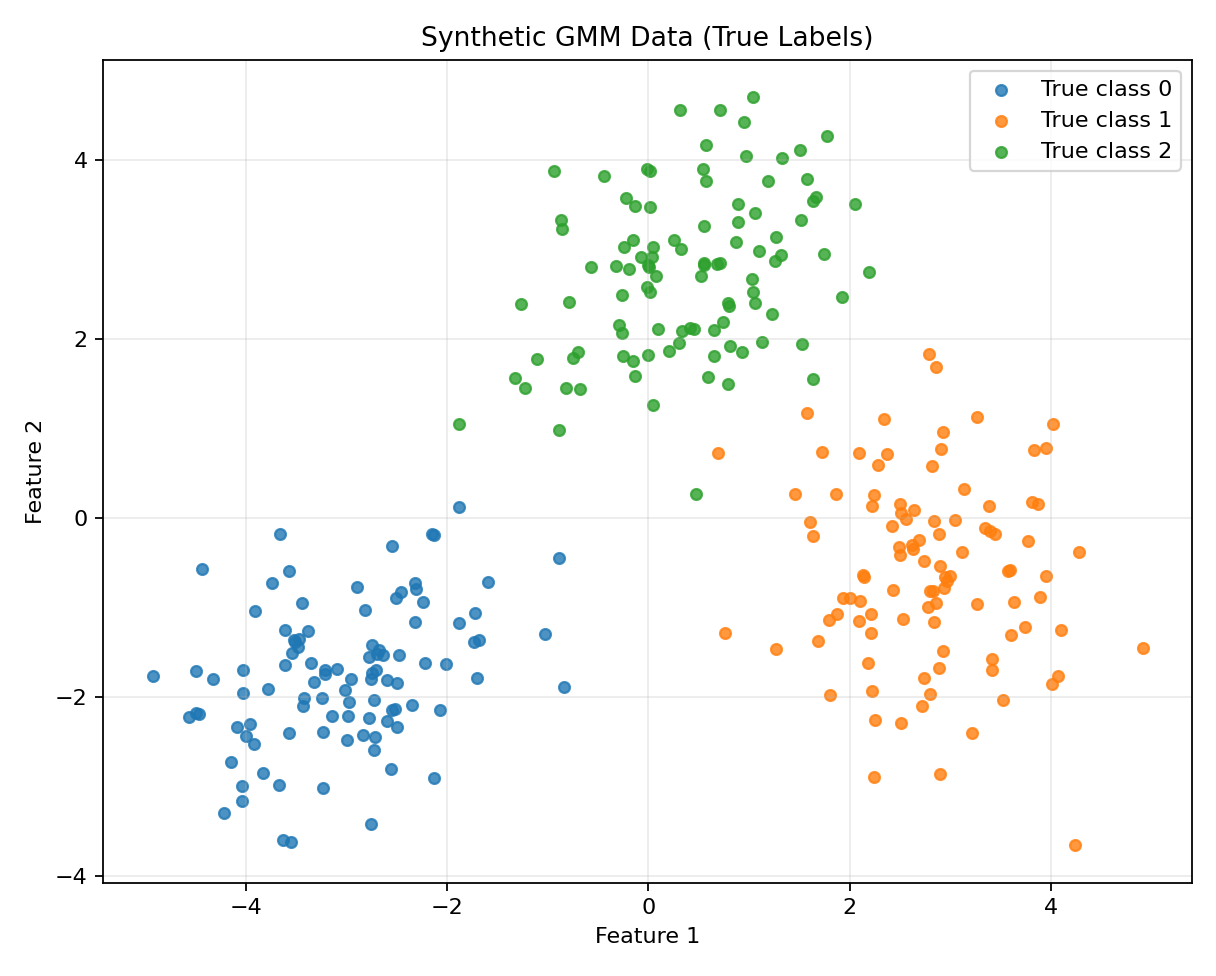
\includegraphics[width=0.82\textwidth]{origin_data.png}
	\caption{混合高斯模拟数据（真实标签）}
\end{figure}

\begin{figure}[H]
	\centering
	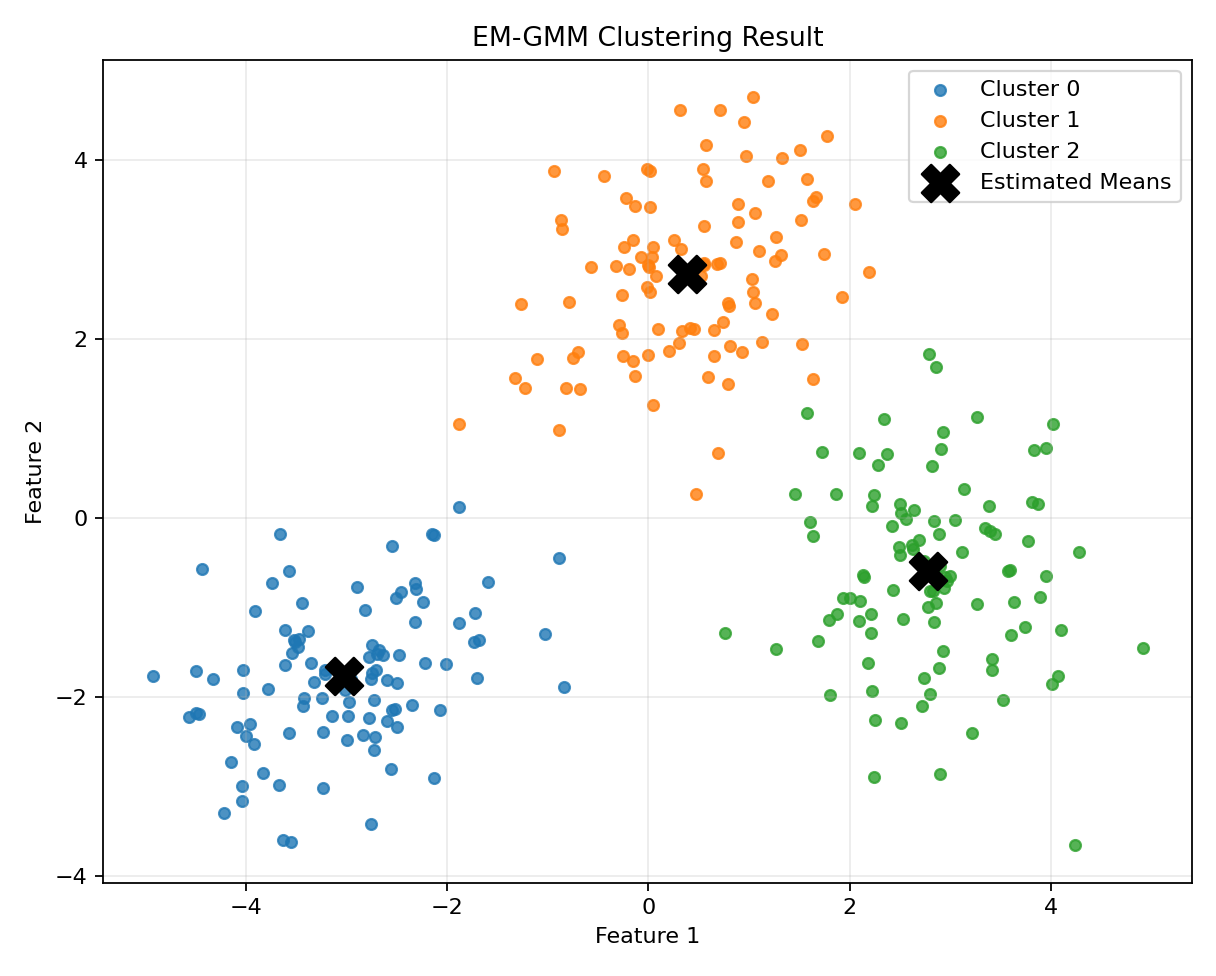
\includegraphics[width=0.84\textwidth]{cluster_output.png}
	\caption{EM-GMM 聚类结果与估计均值}
\end{figure}

\begin{figure}[H]
	\centering
	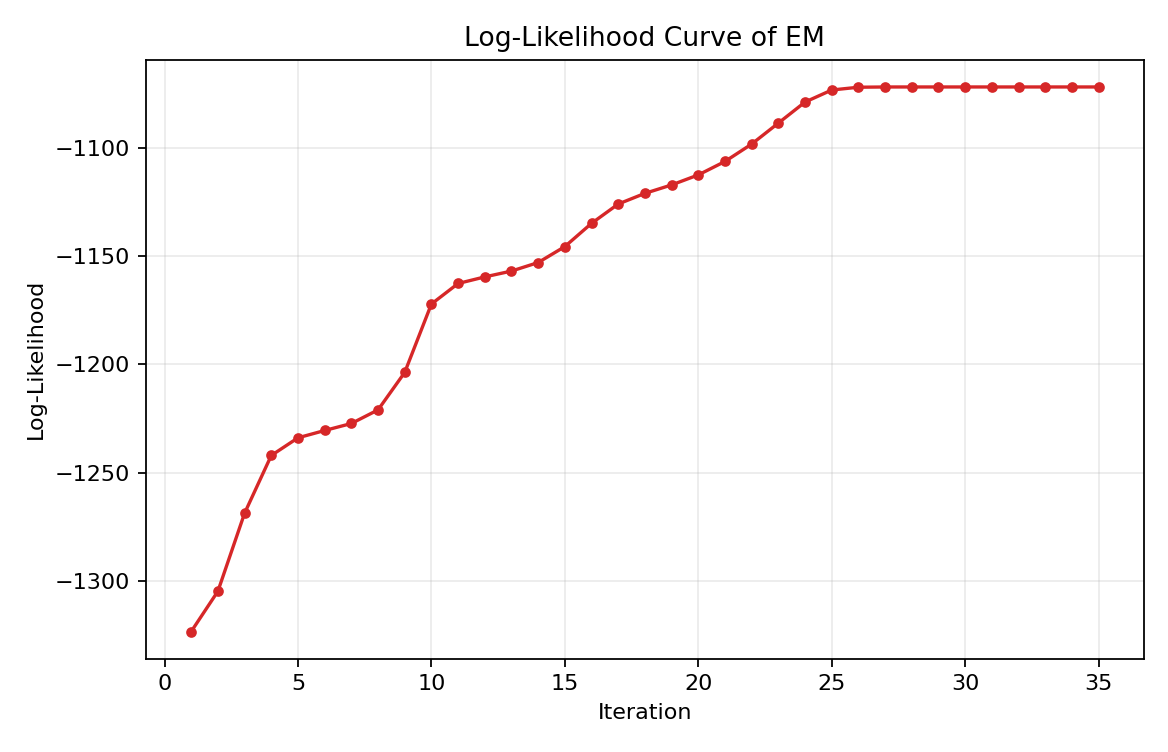
\includegraphics[width=0.78\textwidth]{log_likelihood_curve.png}
	\caption{EM 迭代过程中的对数似然曲线}
\end{figure}

\section*{六、实验中遇到的问题与处理}
\begin{enumerate}
	\item 数值稳定性问题：协方差矩阵可能接近奇异，计算密度时容易不稳定。处理方法是在协方差对角线上加很小的正则项。
	\item 下溢问题：直接连乘概率会非常小，容易造成数值下溢。实验中用对数似然作为收敛指标并在密度求和处做下界截断。
	\item 标签无序问题：聚类标签编号与真实标签编号不一定一致，若直接比较会低估准确率。这里通过全排列匹配取最优映射后再计算准确率。
\end{enumerate}

\section*{七、实验总结}
本次实验从零实现了 EM 算法在 GMM 聚类中的完整流程，包括模型参数初始化、E 步与 M 步迭代、收敛判断和结果评估。实验结果表明，手写实现可以稳定收敛并得到较好的聚类效果。


\end{document}